\section{SNR Estimation} \label{sec:snr_estimation}
The SNR estimation is used for a few subsystems. The Voice Ativity Detection in Section \ref{sec:vad} and the Target Estimation for the Wiener filter in Section \ref{sec:target_estimation}. There are two main approaches to estimate the SNR, these are discussed in this Section.
First the definition of the SNR is written down in Eq. \ref{eq:SNR}. The SNR is the power of the signal divided by the power of the noise. Often, this is expressed in decibel.

\begin{equation}
  \xi = \frac{\sigma_{S,k}(l)^{2}}{\sigma_{N,k}(l)^{2}} =
  \frac{P_{SS,k}}{P_{NN,k}} =
  \frac{E\left\{\abs{S_{k}(l)}^{2}\right\}}{E\left\{\abs{N_{k}(l)}^{2}\right\}}
  \label{eq:SNR}
\end{equation}

\subsection{Maximum Likelihood}
The first estimation approach is based on the maximum likelihood. Here, the signal power is estimated by the Bartlett estimate of the input power. The expected value of the noise power is divided by the order of the Bartlett estimate to use as the denominator.

\begin{align}
  \xi_{k}(l) &= \frac{E\left\{\abs{Y_{k}(l)}^{2}\right\}}{E\left\{\abs{N_{k}(l)}^{2}\right\}} - 1
  \label{eq:ML1}\\
  &= \frac{\hat P_{YY,k}^{B}(l)}{\frac{1}{L}E\left\{\abs{N_{k}(l)}^{2}\right\}}
  \label{eq:M2}
\end{align}

The first testresults of the estimator can be seen in Fig. \ref{fig:mlsnr}. The plot does not include the SNR lower than 0. The SNR estimates are not accurate since the SNR in the test was set at 20dB and the mean of the SNR estimates was 12dB. During speechless periods, it dit give a very small SNR estimate. This could be used as a good indicator for the VAD system.

\begin{figure}[h]
  \centering
  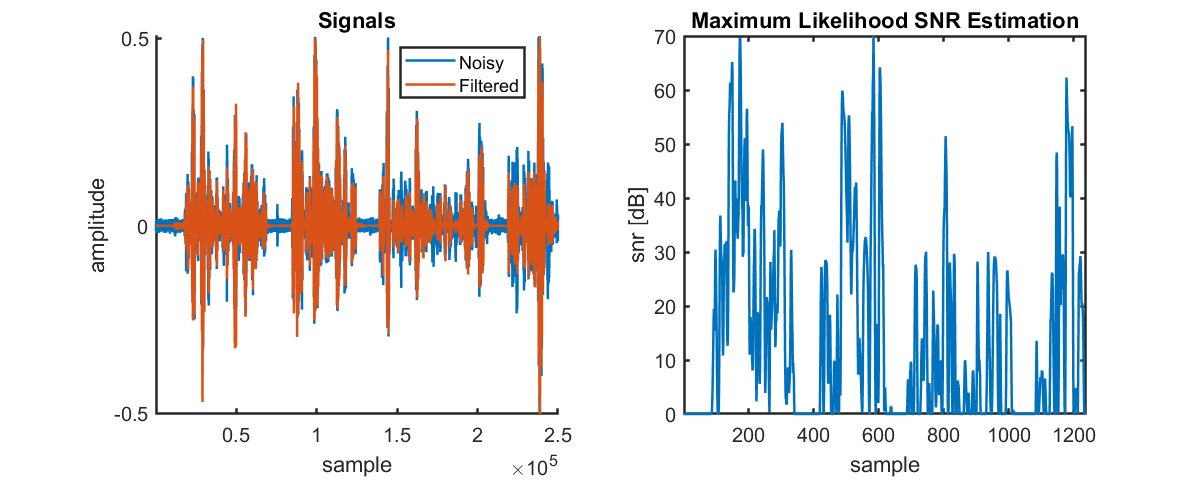
\includegraphics[width=\textwidth]{images/mlsnr.png}
  \caption{SNR Estimation using the ML approach.}
  \label{fig:mlsnr}
\end{figure}

\newpage
\subsection{Decision Directed}
The second estimation approach is more practical. The decision directed approach is making a current SNR estimation with the estimation from the previous frame. A smoothing variable $\alpha$ is used. This can be seen in Eq. \ref{eq:dd1}. Assumed is that the previous SNR estimate is known. The current SNR estimate is using the equations found in Eq. \ref{eq:dd2} and \ref{eq:dd3}.


\begin{align}
  \xi_{k}(l) &= \alpha \frac{E\left\{\abs{S_{k}(l)}^{2}\right\}}{E\left\{\abs{N_{k}(l)}^{2}\right\}} +
  (1-\alpha)\left(\frac{E\left\{\abs{Y_{k}(l)}^{2}\right\}}{E\left\{\abs{N_{k}(l)}^{2}\right\}} - 1\right)
  \label{eq:dd1}\\
  \abs{S_{k}(l)}^{2} &= \abs{\hat S_{k}(l-1)}^{2}
  \label{eq:dd2} \\
  \frac{E\left\{\abs{Y_{k}(l)}^{2}\right\}}{E\left\{\abs{N_{k}(l)}^{2}\right\}} - 1 &=
  \max \left[(\frac{\abs{Y_{k}(l)}^{2}}{E\left\{\abs{N_{k}(l)}^{2}\right\}}-1,0)\right]
  \label{eq:dd3}
\end{align}

The results of the implemented estimator are shown in Fig. \ref{fig:ddsnr}. In comparison to the ML approach, the estimation is much smoother as expected. The areas of speech are more defined. The average SNR on all frames was close to the SNR set on the variables of the model.

\begin{figure}[h]
  \centering
  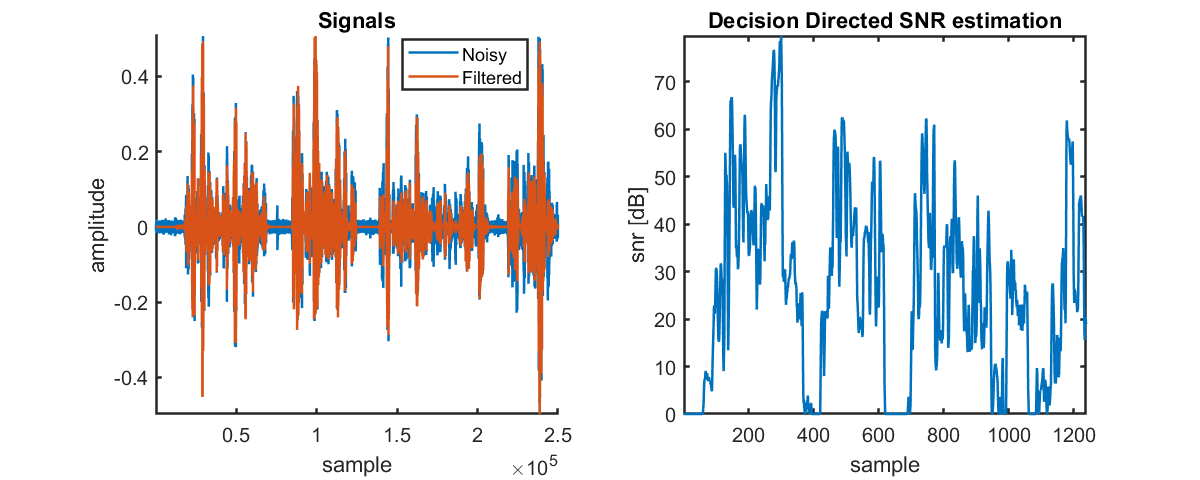
\includegraphics[width=\textwidth]{images/ddsnr.png}
  \caption{SNR Estimation using the DD approach.}
  \label{fig:ddsnr}
\end{figure}
